\documentclass[conference]{IEEEtran}

\usepackage{cite}
\usepackage{amsmath,amssymb}
\usepackage{graphicx}
\usepackage{booktabs}
\usepackage[table]{xcolor}
\usepackage{tikz}
\usetikzlibrary{arrows.meta,positioning,fit,calc}
\usepackage{pgfplots}
\pgfplotsset{compat=1.18, every axis/.append style={font=\scriptsize}}
\usepackage{microtype}
\usepackage{flushend}
\usepackage{url}
\usepackage{hyperref}
\hypersetup{hidelinks,breaklinks=true}

% Tight float gaps: IEEEtran defaults leave large holes under figure*.
\setlength{\textfloatsep}{8pt plus 2pt minus 3pt}
\setlength{\dbltextfloatsep}{8pt plus 2pt minus 3pt}
\setlength{\floatsep}{6pt plus 2pt minus 2pt}
\setlength{\intextsep}{6pt plus 2pt minus 2pt}
\setlength{\abovecaptionskip}{4pt}
\setlength{\belowcaptionskip}{1pt}

\newcommand{\silk}{\textsc{silk}}
\newcommand{\sys}{\emph{Leafmates}}
\newcommand{\pred}[1]{\texttt{#1}}
\newcommand{\dimlab}{\sffamily\tiny\color{labgray}}

\definecolor{headgray}{gray}{0.84}
\definecolor{rowgray}{gray}{0.92}
\definecolor{fillbox}{gray}{0.88}
\definecolor{fillkey}{gray}{0.76}
\definecolor{linegray}{gray}{0.38}
\definecolor{labgray}{gray}{0.32}

\tikzset{
  >=Latex,
  silkarr/.style={-{Latex[length=3.2pt]}, line width=0.55pt, draw=linegray},
  silkbox/.style={
    draw=black!55, fill=fillbox, rounded corners=1.4pt,
    align=center, inner sep=3pt, minimum height=7.6mm,
    font=\sffamily\scriptsize, line width=0.4pt
  },
  silkkey/.style={silkbox, fill=fillkey},
  silknum/.style={
    circle, draw=black!50, fill=fillbox, minimum size=5.6mm,
    inner sep=0pt, font=\sffamily\scriptsize\bfseries, line width=0.4pt
  },
  silklab/.style={font=\sffamily\tiny, text=labgray, align=center},
  callout/.style={
    circle, draw=black, fill=white, minimum size=5.0mm,
    inner sep=0pt, font=\sffamily\scriptsize\bfseries, line width=0.75pt
  },
  pinline/.style={black, line width=0.45pt, -{Stealth[length=1.5mm]}}
}

\begin{document}

\title{Leafmates: Together by Isolation}

\author{\IEEEauthorblockN{Jin Foo}
\IEEEauthorblockA{School of Computing\\
Macquarie University\\
Sydney, Australia\\
eujin.foo@hdr.mq.edu.au}
\and
\IEEEauthorblockN{Amin Beheshti}
\IEEEauthorblockA{School of Computing\\
Macquarie University\\
Sydney, Australia\\
amin.beheshti@mq.edu.au}
\and
\IEEEauthorblockN{Xuyun Zhang}
\IEEEauthorblockA{School of Computing\\
Macquarie University\\
Sydney, Australia\\
xuyun.zhang@mq.edu.au}
}

\maketitle

\begin{abstract}
Isolation-kernel retrieval represents each point as a set of tree leaves. The fraction of shared leaves defines a similarity; \emph{leafmates} are the points isolation failed to cut apart. MinHash and locality-sensitive hashing (LSH) retrieve them in sublinear time after a one-shot encoding. A namespaced leaf, a path of predicates, a band hit, a candidate set, and the exact top-$8$ banding missed are rarely shown together. A visitor should be able to treat the kernel as a readable neighbourhood, not a score. We built a self-contained, network-free explorer, namely \sys{}, and walk it on public simulated spend tables. A visitor may click a travel row, read $\Phi(x)$, hover a leaf for its path, watch LSH admit candidates, and see missed exact leafmates as hollow marks in named spend-category territories. Class labels colour the map; they are not retrieval features.
\end{abstract}

\begin{IEEEkeywords}
Isolation kernel, MinHash, LSH, interactive visualisation, tabular data
\end{IEEEkeywords}

\section{Introduction}

An isolation forest~\cite{Liu2008IsolationForest} assigns each point a leaf in every tree. Two points are similar when they share many of those leaves: that is the isolation kernel~\cite{Ting2018IK}. The fraction of shared leaves defines a similarity. Two points that share them are \emph{leafmates}: isolation grouped them by failing to cut them apart. The kernel is a monotone function of Jaccard overlap on the leaf sets, so MinHash~\cite{Broder1997} estimates it and LSH~\cite{Indyk1998,Leskovec2020MMDS} retrieves candidates in sublinear time after a one-shot encoding. We call the retrieval pipeline \silk{} (isolation-kernel LSH $k$NN).

Decision Predicate Graphs render an isolation forest as a \emph{global} graph of predicates for anomaly isolation~\cite{Ceschin2025DPG}; they do not inspect one query's leafmates, band hits, or the exact neighbours banding missed. LSHiForest treats isolation trees as an LSH ensemble for anomaly analysis~\cite{Zhang2017LSHiForest}, not as an instance-level neighbourhood inspector. Recent isolation-kernel results still target nearest-neighbour search and SVM classification~\cite{Ting2024NN}; $k$NN explainers take a feature-perspective on Euclidean neighbours~\cite{Barcelo2025kNN}. Neither shows a namespaced leaf set, a band hit, and the exact top-$8$ banding missed on one screen. LSH is taught as an S-curve of collision probability against similarity~\cite{Leskovec2020MMDS}, with no corpus under the curve. A scatter of amount against hour shows input geometry, not a leaf or a band hit. The research problem is instance-level inspection of isolation-kernel retrieval. We present a self-contained explorer, namely \sys{}, on public simulated spend tables~\cite{Harris2016Sparkov,Padhi2021TabFormer}: a visitor asks why a travel row retrieved these leafmates, and which exact leafmates LSH did not admit.

The system enables a visitor to: (i)~keep spend-category territories on screen while a dock steps through leaf set, MinHash, LSH, neighbour lock, and tree-prefix overlap; (ii)~read a leaf as a path of predicates and see who shares it; (iii)~compare LSH candidates, ranked by exact shared-leaf count, with the exact top-$8$ by the same order that banding missed; (iv)~read $P(\mathrm{same\ class}\mid\mathrm{shared\ leaves})$ as a measurement on the exported sample, with pair counts, rather than as an assertion. Hover is the join: the same leaf token lights the dock, territory co-members, an inspector row, and the curve.

\section{System}
\label{sec:system}

We present \sys{}, an explorer that makes each stage of the \silk{} path inspectable (Fig.~\ref{fig:pipe}). Let $\Phi(x)=\{(j,\ell_j(x)):j=1,\ldots,t\}$ be the namespaced leaves of $x$ in a forest of $t$ trees. Every point occupies exactly one leaf per tree, so $|\Phi(x)|=t$ for every $x$. Write $c(x,y)=|\Phi(x)\cap\Phi(y)|$. The isolation-kernel fraction is $K=c/t$; Jaccard is $J=c/(2t-c)$. Because every set has size $t$, ranking by $c$, by $K$, and by $J$ coincide: the explorer reports shared-leaf counts and calls the order the exact Jaccard order. Isolation trees cut the feature plane; leafmates are the points those cuts failed to separate (Fig.~\ref{fig:tbi}).

Fig.~\ref{fig:pipe} is the inspectable path. (a)~A leaf is a path of axis-parallel cuts; $\Phi(q)$ is the set of $t$ such leaves, hashed as a set rather than as an embedding vector. (b)~MinHash compresses $\Phi$ to a signature; a whole band of $r{=}3$ rows must match to admit a candidate. Ranking inside $\mathcal{C}$ is the exact shared-leaf count, not the hash. (c)~The three Sparkov travel rows sit in $\mathcal{C}$ for the mechanism seed. LSH admitted them through \emph{different} matching bands---the union of buckets, not one shared bucket---on numeric cuts. No merchant name enters $\Phi$. Class labels colour the map; they are not isolation-forest features, MinHash input, LSH keys, or ranking features. (d)~MinHash and LSH admit $\mathcal{C}$; they do not rank it. The explorer ranks $\mathcal{C}$ by exact shared-leaf count (ties by point id) and draws $N^{\mathrm{exact}}_8\setminus\mathcal{C}$ as a hollow overlay. This seed has four misses; panel~(d) shows the loudest (exact rank~$1$). Missed points were not retrieved.

\begin{figure*}[t]
\centering
% Four-column SILK path (grayscale, IEEE print). Designed at native \textwidth
% (516pt = 181.4mm); total width below is 180.6mm, so no \resizebox is needed.
% Panel (d) is the explorer lock, not a symbolic decision-list rule.
% Note: never name a style "step" (pgfkeys reserved) -- eyebrow style is "eyeb".
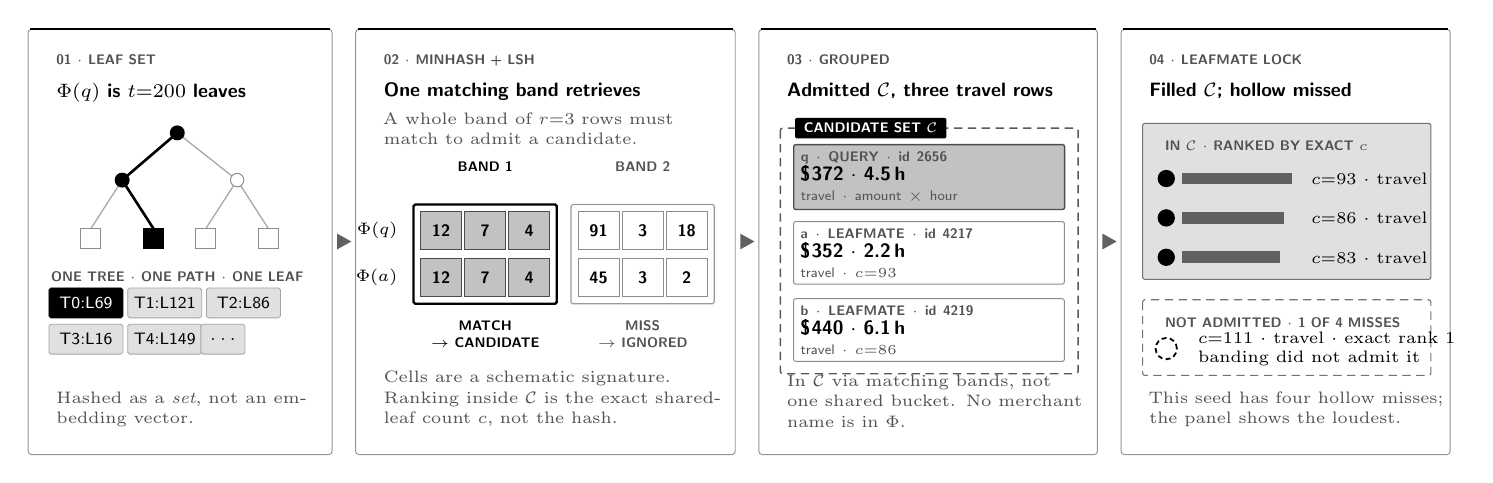
\begin{tikzpicture}[
  x=1mm, y=1mm,
  pan/.style={
    draw=black!42, fill=white, rounded corners=1.2pt,
    line width=0.35pt, inner sep=0pt, anchor=north west
  },
  eyeb/.style={font=\sffamily\fontsize{5.4}{6.0}\selectfont\bfseries, text=labgray},
  hd/.style={font=\sffamily\fontsize{7.4}{8.4}\selectfont\bfseries, text=black},
  gl/.style={font=\fontsize{6.4}{7.4}\selectfont, text=labgray, align=left},
  micro/.style={font=\sffamily\fontsize{5.4}{6.0}\selectfont\bfseries, text=labgray},
  microk/.style={micro, text=black},
  cell/.style={
    draw=black!45, minimum width=5.2mm, minimum height=4.8mm, inner sep=0pt,
    font=\sffamily\fontsize{6.2}{6.6}\selectfont\bfseries, line width=0.35pt
  },
  hit/.style={cell, fill=fillkey, draw=black!70},
  miss/.style={cell, fill=white},
  % 5.6pt keeps the longest real token (T4:L149) inside a 9.4mm chip, so the
  % 10mm chip pitch still leaves a visible gutter between neighbours.
  chip/.style={
    draw=black!35, fill=fillbox, rounded corners=0.7pt,
    minimum width=9.4mm, minimum height=3.8mm, inner sep=0pt,
    font=\sffamily\fontsize{5.6}{6.0}\selectfont, line width=0.3pt
  },
  chipk/.style={chip, fill=black, draw=black, text=white},
  % explicit \fontsize fixes the node baselineskip; otherwise the card
  % inherits the 10/12pt body leading and grows past the bucket.
  card/.style={
    draw=black!45, fill=white, rounded corners=0.8pt, anchor=north west,
    inner sep=0.9mm, text width=32.6mm, align=left, line width=0.35pt,
    font=\fontsize{5.6}{6.6}\selectfont
  },
  cardq/.style={card, fill=fillkey, draw=black!70, line width=0.5pt},
  rowlab/.style={font=\fontsize{6.2}{7.0}\selectfont, anchor=west}
]

\def\PH{54}      % panel height (mm)
\def\GY{-51.8}   % gloss baseline (anchor south west) inside each panel
\def\AX{0}    \def\AW{38.6}
\def\BX{41.6} \def\BW{48.2}
\def\CX{92.8} \def\CW{43.0}
\def\DX{138.8}\def\DW{41.8}

% ---------- panel shells + top rules ----------
\node[pan, minimum width=\AW mm, minimum height=\PH mm] (A) at (\AX,0) {};
\node[pan, minimum width=\BW mm, minimum height=\PH mm] (B) at (\BX,0) {};
\node[pan, minimum width=\CW mm, minimum height=\PH mm] (C) at (\CX,0) {};
\node[pan, minimum width=\DW mm, minimum height=\PH mm] (D) at (\DX,0) {};
\foreach \n in {A,B,C,D}{%
  \draw[black, line width=0.9pt] ([xshift=0.3mm]\n.north west) -- ([xshift=-0.3mm]\n.north east);}

% ---------- flow chevrons in the gutters ----------
\foreach \gx in {39.3, 90.5, 136.5}{%
  \fill[linegray] (\gx,-26.0) -- (\gx,-28.0) -- (\gx+1.8,-27.0) -- cycle;}

% =========================== (a) leaf set ===========================
\begin{scope}[shift={(\AX,0)}]
  \node[eyeb, anchor=north west] at (2.4,-2.0) {01 $\cdot$ LEAF SET};
  \node[hd, anchor=north west]   at (2.4,-5.6) {$\Phi(q)$ is $t{=}200$ leaves};

  % --- isolation tree: one dark root-to-leaf path, rest light ---
  \draw[black!35, line width=0.45pt] (19.0,-13.2) -- (26.6,-19.2);
  \draw[black!35, line width=0.45pt] (12.0,-19.2) -- (8.0,-25.4);
  \draw[black!35, line width=0.45pt] (26.6,-19.2) -- (22.6,-25.4);
  \draw[black!35, line width=0.45pt] (26.6,-19.2) -- (30.6,-25.4);
  \draw[black, line width=0.95pt]    (19.0,-13.2) -- (12.0,-19.2);
  \draw[black, line width=0.95pt]    (12.0,-19.2) -- (16.0,-25.4);
  % hollow leaves
  \foreach \lx in {8.0, 22.6, 30.6}{%
    \draw[fill=white, draw=black!45, line width=0.35pt]
      (\lx-1.25,-27.85) rectangle (\lx+1.25,-25.35);}
  % selected leaf
  \draw[fill=black, draw=black, line width=0.35pt]
    (14.75,-27.85) rectangle (17.25,-25.35);
  % internal nodes
  \draw[fill=white, draw=black!45, line width=0.35pt] (26.6,-19.2) circle (0.85mm);
  \fill[black] (19.0,-13.2) circle (0.95mm);
  \fill[black] (12.0,-19.2) circle (0.95mm);

  \node[micro, anchor=north] at (19.0,-29.6) {ONE TREE $\cdot$ ONE PATH $\cdot$ ONE LEAF};

  % --- leaf-id chips: Phi(q) is a set of namespaced leaves ---
  % Real fingerprint sample of the mechanism seed (id 2656); the filled chip is
  % the leaf hovered in Fig. 3.
  \node[chipk] at (7.4,-34.8) {T0:L69};
  \node[chip]  at (17.4,-34.8) {T1:L121};
  \node[chip]  at (27.4,-34.8) {T2:L86};
  \node[chip]  at (7.4,-39.4) {T3:L16};
  \node[chip]  at (17.4,-39.4) {T4:L149};
  \node[chip, minimum width=5.6mm] at (24.8,-39.4) {$\ldots$};

  \node[gl, anchor=south west, text width=33.8mm] at (2.4,\GY)
    {Hashed as a \emph{set}, not an embedding vector.};
\end{scope}

% ======================= (b) MinHash + LSH =========================
\begin{scope}[shift={(\BX,0)}]
  \node[eyeb, anchor=north west] at (2.4,-2.0) {02 $\cdot$ MINHASH + LSH};
  \node[hd, anchor=north west]   at (2.4,-5.6) {One matching band retrieves};
  \node[gl, anchor=north west, text width=43.0mm] at (2.4,-9.4)
    {A whole band of $r{=}3$ rows must match to admit a candidate.};

  \node[microk, anchor=south] at (16.5,-19.4) {BAND 1};
  \node[micro,  anchor=south] at (36.5,-19.4) {BAND 2};

  % band frames: the grouping unit, not six loose cells
  \draw[black, line width=0.85pt, rounded corners=0.6pt]
    (7.4,-22.3) rectangle (25.6,-34.9);
  \draw[black!40, line width=0.4pt, rounded corners=0.6pt]
    (27.4,-22.3) rectangle (45.6,-34.9);

  \node[rowlab, anchor=east] at (6.6,-25.6) {$\Phi(q)$};
  \node[rowlab, anchor=east] at (6.6,-31.6) {$\Phi(a)$};

  \node[hit]  at (10.9,-25.6) {12};  \node[hit]  at (16.5,-25.6) {7};
  \node[hit]  at (22.1,-25.6) {4};
  \node[miss] at (30.9,-25.6) {91};  \node[miss] at (36.5,-25.6) {3};
  \node[miss] at (42.1,-25.6) {18};
  \node[hit]  at (10.9,-31.6) {12};  \node[hit]  at (16.5,-31.6) {7};
  \node[hit]  at (22.1,-31.6) {4};
  \node[miss] at (30.9,-31.6) {45};  \node[miss] at (36.5,-31.6) {3};
  \node[miss] at (42.1,-31.6) {2};

  % two lines: a single-line legend is wider than a band and the two collide
  \node[microk, anchor=north, align=center] at (16.5,-35.9)
    {MATCH\\$\rightarrow$ CANDIDATE};
  \node[micro,  anchor=north, align=center] at (36.5,-35.9)
    {MISS\\$\rightarrow$ IGNORED};

  \node[gl, anchor=south west, text width=43.4mm] at (2.4,\GY)
    {Cells are a schematic signature. Ranking inside $\mathcal{C}$ is the exact
     shared-leaf count $c$, not the hash.};
\end{scope}

% ===================== (c) grouped travel rows =====================
\begin{scope}[shift={(\CX,0)}]
  \node[eyeb, anchor=north west] at (2.4,-2.0) {03 $\cdot$ GROUPED};
  \node[hd, anchor=north west]   at (2.4,-5.6) {Admitted $\mathcal{C}$, three travel rows};

  \draw[black!65, line width=0.5pt, densely dashed, rounded corners=0.8pt]
    (2.8,-12.6) rectangle (40.6,-43.8);
  \node[micro, text=white, fill=black, inner xsep=1.1mm, inner ysep=0.7mm,
        rounded corners=0.5pt, anchor=west] at (4.6,-12.6) {CANDIDATE SET $\mathcal{C}$};

  % Sparkov mechanism seed (query 2656) and its top-2 leafmates inside C,
  % rounded for print. Amount x hour only: merchant names are not in Phi.
  \node[cardq] at (4.4,-14.6)
    {{\sffamily\fontsize{5.2}{5.8}\selectfont\bfseries\color{labgray} q $\cdot$ QUERY $\cdot$ id 2656}\\[0.15mm]
     {\sffamily\fontsize{6.6}{7.2}\selectfont\bfseries \$372 $\cdot$ 4.5\,h}\\[0.15mm]
     {\sffamily\fontsize{5.4}{6.0}\selectfont\color{labgray} travel $\cdot$ amount $\times$ hour}};
  \node[card] at (4.4,-24.4)
    {{\sffamily\fontsize{5.2}{5.8}\selectfont\bfseries\color{labgray} a $\cdot$ LEAFMATE $\cdot$ id 4217}\\[0.15mm]
     {\sffamily\fontsize{6.6}{7.2}\selectfont\bfseries \$352 $\cdot$ 2.2\,h}\\[0.15mm]
     {\sffamily\fontsize{5.4}{6.0}\selectfont\color{labgray} travel $\cdot$ $c{=}93$}};
  \node[card] at (4.4,-34.2)
    {{\sffamily\fontsize{5.2}{5.8}\selectfont\bfseries\color{labgray} b $\cdot$ LEAFMATE $\cdot$ id 4219}\\[0.15mm]
     {\sffamily\fontsize{6.6}{7.2}\selectfont\bfseries \$440 $\cdot$ 6.1\,h}\\[0.15mm]
     {\sffamily\fontsize{5.4}{6.0}\selectfont\color{labgray} travel $\cdot$ $c{=}86$}};

  \node[gl, anchor=south west, text width=38.2mm] at (2.4,\GY)
    {In $\mathcal{C}$ via matching bands, not one shared bucket. No merchant name is in $\Phi$.};
\end{scope}

% ========================= (d) ranked lock =========================
\begin{scope}[shift={(\DX,0)}]
  \node[eyeb, anchor=north west] at (2.4,-2.0) {04 $\cdot$ LEAFMATE LOCK};
  \node[hd, anchor=north west]   at (2.4,-5.6) {Filled $\mathcal{C}$; hollow missed};

  % admitted + ranked
  \draw[black!55, fill=fillbox, line width=0.4pt, rounded corners=0.8pt]
    (2.8,-12.0) rectangle (39.4,-31.8);
  \node[micro, anchor=north west] at (4.4,-13.0) {IN $\mathcal{C}$ $\cdot$ RANKED BY EXACT $c$};
  % Bars are c scaled against the admitted maximum (93 -> 14.0mm); 111 is not
  % drawn as a bar because it would run past the panel.
  \foreach \yy/\bw/\cv in {-19.0/14.0/93, -24.0/12.9/86, -29.0/12.5/83}{%
    \fill[black] (5.8,\yy) circle (1.1mm);
    \fill[black!62] (7.8,\yy-0.75) rectangle (7.8+\bw,\yy+0.75);
    \node[font=\fontsize{6.2}{7.0}\selectfont, anchor=west] at (23.0,\yy)
      {$c{=}\cv$ $\cdot$ travel};}

  % missed by banding
  \draw[black!55, fill=white, line width=0.4pt, densely dashed, rounded corners=0.8pt]
    (2.8,-34.4) rectangle (39.4,-44.0);
  \node[micro, anchor=north west] at (4.4,-35.4) {NOT ADMITTED $\cdot$ 1 OF 4 MISSES};
  \draw[black, line width=0.65pt, dash pattern=on 0.62mm off 0.42mm]
    (5.8,-40.6) circle (1.35mm);
  \node[font=\fontsize{6.2}{7.0}\selectfont, anchor=west, align=left] at (8.6,-40.6)
    {$c{=}111$ $\cdot$ travel $\cdot$ exact rank 1\\banding did not admit it};

  \node[gl, anchor=south west, text width=37.0mm] at (2.4,\GY)
    {This seed has four hollow misses; the panel shows the loudest.};
\end{scope}

\end{tikzpicture}

\caption{\silk{} path the explorer makes inspectable. (a)~$\Phi(q)$ is $t{=}200$ namespaced leaves; a leaf is a path. (b)~A matching band of $r{=}3$ admits a candidate; a miss is ignored. (c)~Mechanism-seed travel rows in $\mathcal{C}$ (not one bucket), amount ${\times}$ hour, rounded; the Wow-path seed of Sec.~\ref{sec:demo}. (d)~Filled: $\mathcal{C}$ ranked by exact $c$; hollow: one of four $N^{\mathrm{exact}}_8\setminus\mathcal{C}$ misses. Packed HTML (open locally): \href{https://github.com/jin-foo/2026-JinFOO-Demo-ICDM}{\texttt{github.com/jin-foo/2026-JinFOO-Demo-ICDM}}.}
\label{fig:pipe}
\end{figure*}

\begin{figure*}[!t]
\centering
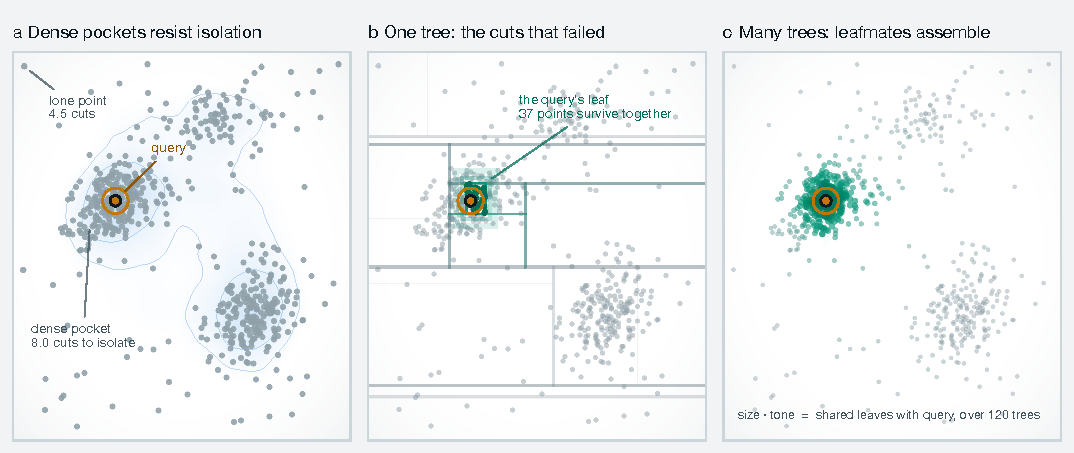
\includegraphics[width=\textwidth]{figures/together-by-isolation.pdf}
\caption{Together by isolation (schematic 2-D feature plane, not a projection of $\Phi$). (a)~Isolation depth wash: dense pockets take more random cuts; a lone point falls out early. (b)~One tree: the query's leaf cell is outlined and the darker points inside it are its leafmates---the cuts that failed. (c)~Kernel field: shared-leaf fraction with the query across a schematic forest (booth artefacts use $t{=}200$). Size and tone encode the same count. Isolation is the grouping operator.}
\label{fig:tbi}
\end{figure*}

A Python exporter fits $t{=}200$ trees (max depth $16$, subsample $256$), $H{=}120$ MinHash functions, and $B{=}40$ bands of $r{=}3$ rows, then writes JSON (\texttt{schema} v4, \texttt{random\_state=42}): amount${}\times{}$hour coordinates, exact shared-leaf top-$8$, LSH candidate lists, missed exact neighbours, isolation paths as $(\mathrm{feature},\mathrm{op},\mathrm{value})$, and a pooled overlap histogram. The browser never fits a forest. Inspection is client-side on the packed HTML, which makes no network request. The companion repository is \url{https://github.com/jin-foo/2026-JinFOO-Demo-ICDM} (\texttt{demo/leafmates.html}; download and open locally---GitHub does not execute it). Hover is the linking operator among canvas, dock, inspector, and curve.

\section{Demonstration Scenario}
\label{sec:demo}

The demonstration scenario assists a visitor who has selected a travel spend row and wants to know \emph{why} isolation-kernel retrieval returned these leafmates, and which exact leafmates LSH did not admit. Class labels colour the map; they are not isolation-forest features, MinHash input, LSH keys, or ranking features. Territories group classes for explanation; dots inside a region are a deterministic sample, not a projection of $\Phi$. We demonstrate the explorer in Fig.~\ref{fig:ui} along a six-step walk (cloud, leaves, MinHash, LSH, lock, overlap). The packed HTML is linked from Fig.~\ref{fig:pipe}.

The guided path uses the Sparkov \emph{mechanism} seed (travel; $78$ candidates, $98.7\%$ reduction, four exact top-$8$ misses, candidate-set purity $0.75$). It is the seed the booth Wow button runs, and it keeps several class territories on screen. Twenty-four exported queries pulse on the idle canvas; three named roles (mechanism, pure, mixed) are a presenter shortcut. A visitor may click any pulsing seed, including neighbourhoods that are mostly off-class.

\begin{figure*}[!t]
\centering
\begin{minipage}{0.96\linewidth}
\centering
\begin{tikzpicture}
\node[inner sep=0] (ui) {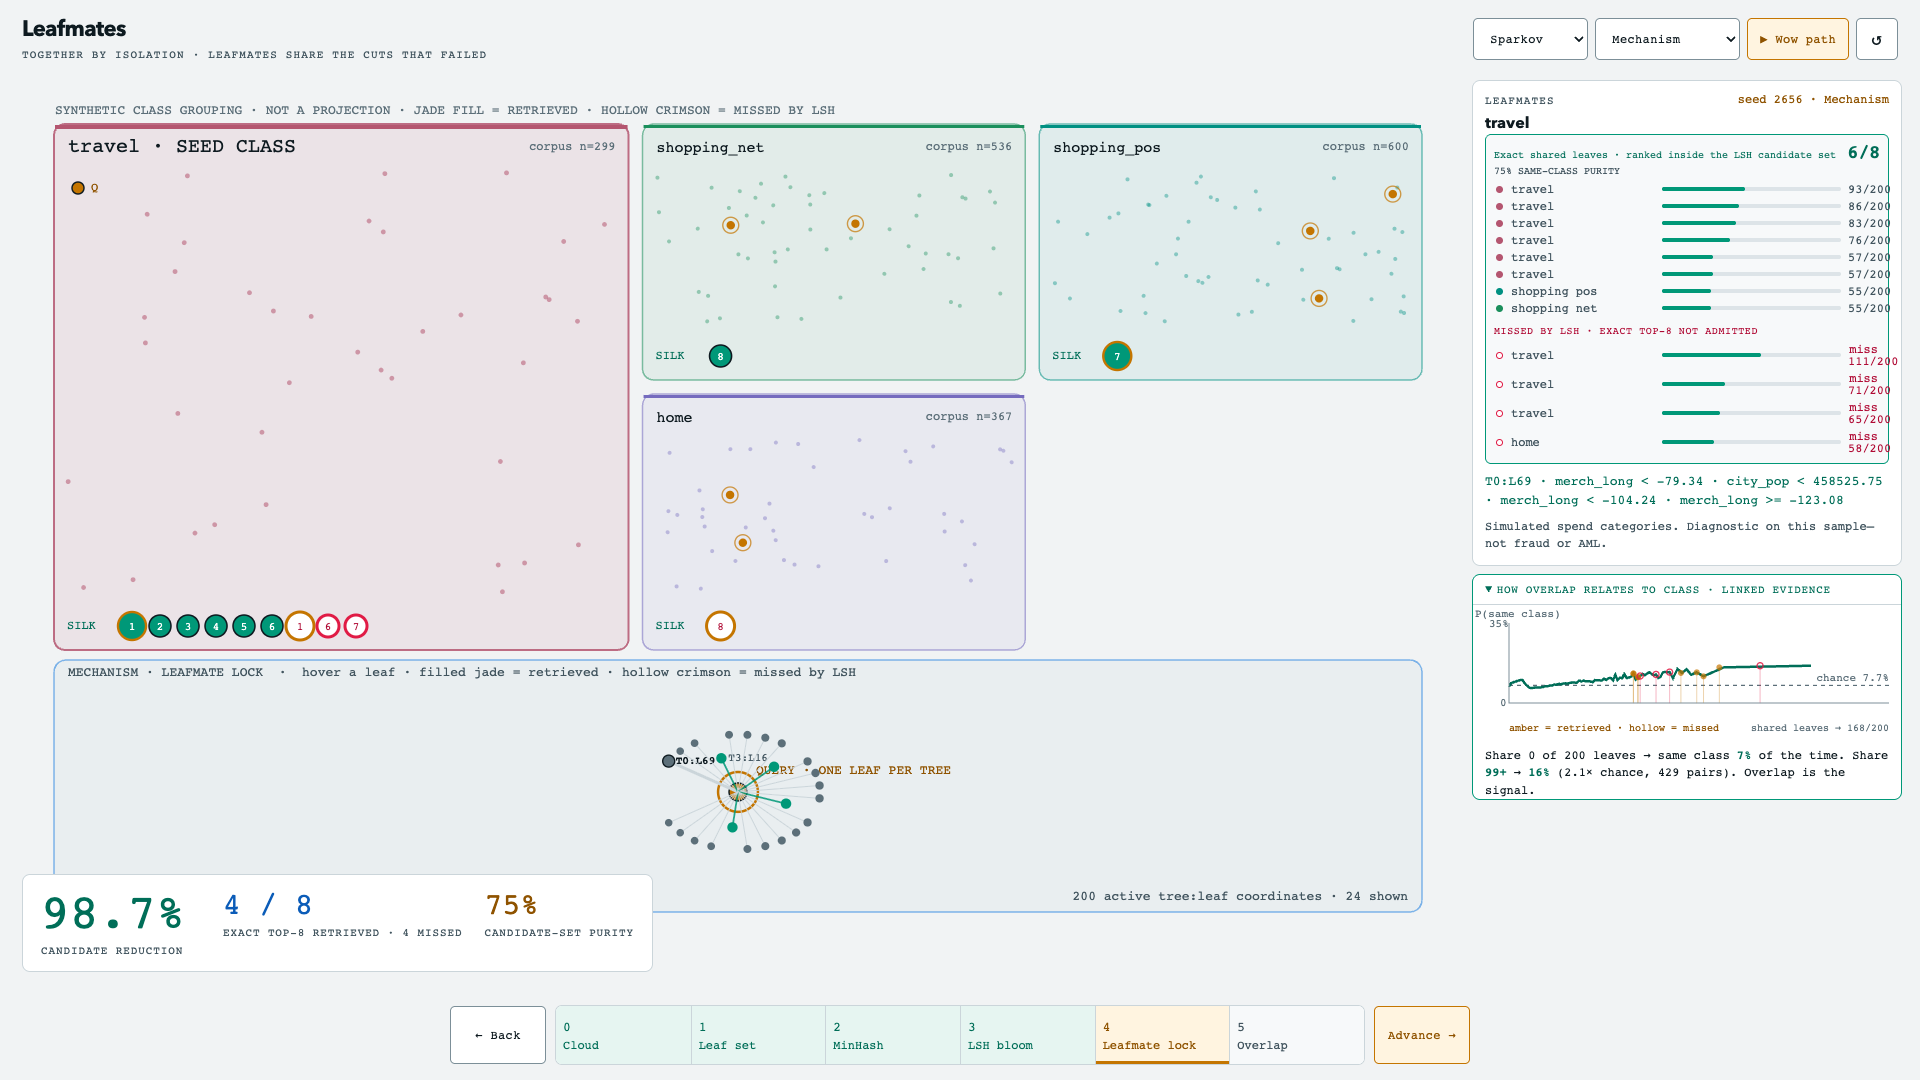
\includegraphics[width=\linewidth]{figures/ui-annotated.png}};
% Offsets: callout circle (offset so it does not sit on the target) then a
% short pin to the named object. Scale 174.26mm / 1920px.
% Pins: markers (258,626); ring (738,792); predicate (1485,472);
% list (1510,220); amp-read (1687,760).
\node[callout] (c1) at ([xshift=14.0mm,yshift=-48.0mm]ui.north west) {1};
\draw[pinline] (c1) -- ([xshift=23.4mm,yshift=-56.8mm]ui.north west);
\node[callout] (c2) at ([xshift=54.0mm,yshift=-62.0mm]ui.north west) {2};
\draw[pinline] (c2) -- ([xshift=67.0mm,yshift=-71.9mm]ui.north west);
\node[callout] (c3) at ([xshift=124.0mm,yshift=-40.0mm]ui.north west) {3};
\draw[pinline] (c3) -- ([xshift=136.2mm,yshift=-44.1mm]ui.north west);
\node[callout] (c4) at ([xshift=124.0mm,yshift=-17.0mm]ui.north west) {4};
\draw[pinline] (c4) -- ([xshift=137.0mm,yshift=-22.0mm]ui.north west);
\node[callout] (c5) at ([xshift=124.0mm,yshift=-61.0mm]ui.north west) {5};
\draw[pinline] (c5) -- ([xshift=153.1mm,yshift=-68.3mm]ui.north west);
\end{tikzpicture}
\caption{Snapshot of the explorer on Sparkov, mechanism seed, leafmate-lock stage, with leaf \texttt{T0:L69} hovered. (1)~Seed-class territory: query and ranked leafmates (filled) plus misses (hollow) lock on class. (2)~Dock: $24$ of $200$ leaves; the hovered leaf is marked. (3)~Path predicates for that leaf. (4)~Inspector: exact shared-leaf rank inside $\mathcal{C}$, and the four exact top-$8$ LSH missed. (5)~Overlap curve $P(\mathrm{same\ class}\mid\mathrm{shared\ leaves})$; pair counts are in the curve readout.}
\label{fig:ui}
\end{minipage}
\end{figure*}

\textbf{Step 0 (cloud).} \emph{Does:} click a pulsing seed, or start the guided path. \emph{Learns:} the idle canvas is amount against hour, coloured by spend category. Labels paint the map; they are not features.

\textbf{Step 1 (leaves).} \emph{Does:} hover a leaf in the dock. \emph{Learns:} the row is $\Phi(x)$, one leaf per tree. The dock shows a sample of $24$ leaves from $t{=}200$. Hover prints a conjunction of axis-aligned predicates---e.g.\ \pred{merch\_long < -79.34}, \pred{city\_pop < 458526}, \pred{merch\_long < -104.24}---and lights co-members. A leaf is a path, not a single split. Territories for the seed class and its neighbours lock above and stay.

\textbf{Step 2 (MinHash).} \emph{Does:} watch the dock compress $\Phi(x)$ to $H{=}120$ hash values. \emph{Learns:} matching bands (whole $r{=}3$ rows) are what will admit candidates. MinHash does not rank.

\textbf{Step 3 (LSH).} \emph{Does:} watch matching bands bloom into the territories. \emph{Learns:} on this seed, $78$ of $6{,}000$ points remain as candidates ($98.7\%$ reduction). LSH admits $\mathcal{C}$; ranking comes next.

\textbf{Step 4 (lock).} \emph{Does:} hover a filled or hollow marker. \emph{Learns:} filled markers are $\mathcal{C}$ ranked by exact shared-leaf count. Hollow markers are the exact top-$8$ by that order that banding did not admit---an overlay, not retrieved neighbours. Hover lights shared leaves and moves the curve readout.

\textbf{Step 5 (overlap).} \emph{Does:} read the inspector curve and the tree-prefix dock. \emph{Learns:} ranking never uses labels. The curve is post-hoc association, $P(\mathrm{same\ class}\mid\mathrm{shared\ leaves})$, with pair counts because the high-overlap tail is thin. On this seed the exact top-$8$ purity rises from $0$ with one tree to $0.875$ with $200$; the pooled tree-prefix curve on the sample barely moves, which is why the booth reports the measured overlap curve rather than a vote story.

The mixed grocery seed (purity $0.50$) is the honesty check: off-class leafmates in shopping and misc, no hollow misses, same dock and inspector. The pure travel seed (purity $1.00$, $23$ candidates, five misses) remains in the dropdown so a presenter can show a single-class neighbourhood without pretending it is typical. The 90-second booth path is Fig.~\ref{fig:pipe} then hover: a visitor should leave able to read a leaf as a path, a matching band, a filled candidate, and a hollow miss.

\section{Observations}

Table~\ref{tab:diag} reports all $6{,}000$ exported points. Column ``purity'' is the mean same-class fraction in the MinHash-estimated Jaccard top-$8$ ($0.16$ / $0.23$). The HUD reports a different number: candidate-set purity, the same-class fraction among the exact shared-leaf ranking \emph{inside} $\mathcal{C}$. On the mechanism seed those values are $1.00$ and $0.75$; they are not two readings of Table~\ref{tab:diag}. Candidate recall@8 is $|\mathcal{C}_i\cap N^{\mathrm{exact}}_8(i)|/8$, averaged over every point, where $N^{\mathrm{exact}}_8(i)$ is the exact shared-leaf top-$8$ (ties by id). LSH keeps about half of those neighbours on Sparkov ($0.56$) and almost all of them on TabFormer ($0.998$), where buckets are wide: $80\%$ of TabFormer queries hit a deterministic cap of $500$, so the reported mean $|\mathcal{C}|=452$ is retained-after-cap, not the uncapped union. Sparkov cap-hit is $0$. No-candidate rates are at or near zero ($0.02\%$ on Sparkov; none of the $24$ pulsing queries is empty). The explorer draws $N^{\mathrm{exact}}_8(i)\setminus\mathcal{C}_i$ as hollow marks.

Fig.~\ref{fig:amp} is the pooled overlap curve. High overlap lifts $P(\mathrm{same\ class})$; the TabFormer chance rate is $9.6\%$. Bins of width $20$ keep the thin tail from looking more certain than its pair counts. Artefacts are precomputed---a visitor inspects a frozen index, not a live encode. Territories are synthetic grouping. TabFormer's near-one recall is bought by wide buckets, not by a tighter index.

\begin{table}[t]
\centering
\caption{Booth artefacts ($t{=}200$, $H{=}120$, $B{=}40\times r{=}3$, $k{=}8$, all $6{,}000$ points). Purity: mean same-class fraction in the MinHash-estimated Jaccard top-$8$. $|\mathcal{C}|$ and rec.@8: LSH candidates retained after a cap of $500$, versus the exact shared-leaf top-$8$.}
\label{tab:diag}
\renewcommand{\arraystretch}{1.22}
\setlength{\tabcolsep}{3.4pt}
\setlength{\aboverulesep}{0pt}
\setlength{\belowrulesep}{0pt}
\begin{tabular}{lrrrrrr}
\toprule
\rowcolor{headgray}
Corpus & $n$ & $d$ & $C$ & purity & $|\mathcal{C}|$ & rec.@8 \\
\midrule
Sparkov~\cite{Harris2016Sparkov} & 6\,000 & 9 & 14 & 0.16 & 41 & 0.56 \\
\rowcolor{rowgray}
TabFormer~\cite{Padhi2021TabFormer} & 6\,000 & 5 & 12 & 0.23 & 452 & 0.998 \\
\bottomrule
\end{tabular}
\end{table}

\begin{figure}[t]
\centering
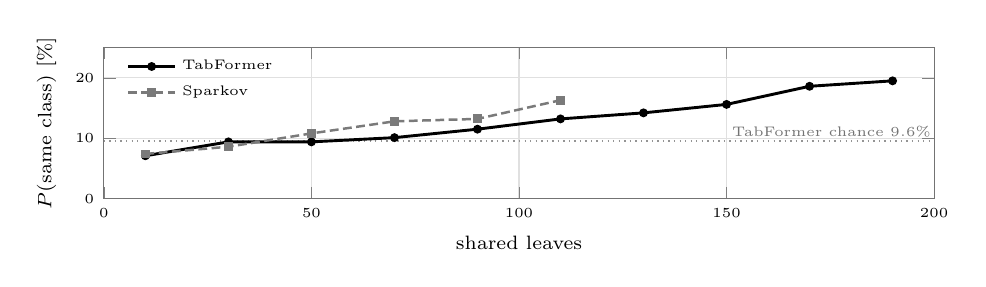
\begin{tikzpicture}
\begin{axis}[
  width=\columnwidth,
  height=3.5cm,
  xlabel={shared leaves},
  ylabel={$P$(same class) [\%]},
  xmin=0, xmax=200,
  ymin=0, ymax=25,
  xtick={0,50,100,150,200},
  ytick={0,10,20},
  % Two entries only, parked in the empty upper-left corner; the chance line
  % is labelled where it runs so it needs no key.
  legend style={font=\tiny, at={(0.025,0.97)}, anchor=north west, draw=none,
                fill=none, inner sep=0.5pt, row sep=0.5pt},
  legend cell align=left,
  tick label style={font=\tiny},
  label style={font=\scriptsize},
  axis line style={black!55},
  tick style={black!50},
  grid=major,
  grid style={black!12},
  clip=false,
]
\addplot[black!42, line width=0.7pt, dash pattern=on 0.5pt off 1.5pt, forget plot]
  coordinates {(0,9.6) (200,9.6)};
\node[anchor=south east, font=\tiny, text=black!55, inner sep=1pt]
  at (axis cs:200,9.6) {TabFormer chance $9.6\%$};
\addplot[black, line width=1.05pt, mark=*, mark size=1.05pt, mark options={fill=black, draw=black, solid}] coordinates {
  (10,7.1) (30,9.4) (50,9.4) (70,10.1) (90,11.5)
  (110,13.2) (130,14.2) (150,15.6) (170,18.6) (190,19.5)
};
\addlegendentry{TabFormer}
\addplot[black!52, dashed, line width=0.9pt, dash pattern=on 3.2pt off 1.6pt,
         mark=square*, mark size=1.15pt,
         mark options={fill=black!52, draw=black!52, solid}] coordinates {
  (10,7.4) (30,8.6) (50,10.8) (70,12.8) (90,13.2) (110,16.3)
};
\addlegendentry{Sparkov}
\end{axis}
\end{tikzpicture}
\caption{$P(\mathrm{same\ class}\mid\mathrm{shared\ leaves})$ on the exported sample, in non-overlapping bins of $20$ shared leaves, plotted at bin centres. High overlap lifts probability; Sparkov stops after the $100$--$119$ bin ($326$ pairs). Chance on TabFormer is $9.6\%$.}
\label{fig:amp}
\end{figure}

\section{Data and ethics}

Both corpora are simulated: schema-matched samples in the Sparkov~\cite{Harris2016Sparkov} and TabFormer~\cite{Padhi2021TabFormer} layouts, not row draws from those public CSVs. The Sparkov shard has fourteen named spend categories; features are amount, hour, day-of-week, customer and merchant coordinates, city population, and gender. Isolation trees may split on gender because it is in the public schema; removing it would misrepresent what the forest saw, and when they split the explorer prints that predicate. TabFormer contributes amount, hour, day-of-week, chip use, and errors; we roll merchant category code (MCC) into twelve groups. Person names, card numbers, merchant names, raw MCC, and fraud flags are dropped. Class is spend category. The explorer shows $6{,}000$ of $50{,}000$-row shards (\texttt{schema} v4, \texttt{random\_state=42}). No personal names, account numbers, or application identifiers appear. No human-subject study is reported. The client is static HTML with both artefacts embedded; it makes no network request.

\section{Conclusion}

Isolation-kernel retrieval is inspectable when the leaf set, the path, the candidate set, and the missed exact neighbours share a screen. \sys{} is a packed, network-free explorer that does this on public simulated spend tables. Hover joins those views. Shared-leaf fraction is the similarity; class labels only colour the map. The packed HTML is linked from Fig.~\ref{fig:pipe}.

The booth constraint is a frozen index: a visitor inspects, they do not re-fit. A useful next engineering step is a live encode on a larger public shard without giving up the network-free pack. This demo stops at inspectability: a visitor should leave the booth able to read $\Phi(x)$, a band hit, and a hollow miss.

\section*{Acknowledgment}
We acknowledge the Centre for Applied Artificial Intelligence at Macquarie University for funding this research. We also acknowledge the use of AI-assisted tools during the preparation of this manuscript, including for editorial refinement and the generation of selected draft content such as statements and figures. All AI-assisted outputs were reviewed, verified, and approved by the authors, who take full responsibility for the final content of the manuscript.

\bibliographystyle{IEEEtran}
\bibliography{references}

\end{document}
